% !TeX spellcheck = es_ES
% !TEX encoding = UTF-8 Unicode
\documentclass[t, compress, spanish, aspectratio=169]{beamer}
%\documentclass[t, compress, spanish]{beamer} % for the presentation
%\documentclass[handout]{beamer}    % for the handout

\usetheme[progressbar=frametitle, subsectionpage=progressbar]{metropolis}

%\usetheme[secheader]{Madrid}
%\usetheme{Frankfurt}
%\usetheme{Warsaw}
%\usetheme{Berlin}
%\usetheme{CambridgeUS}

%\usecolortheme{beaver}     % Fondo Blanco y letras Negras - Titulos en Rojo con fondo gris
%\usecolortheme{dove}       % Para el Handout
%\usecolortheme{seahorse}   % Fondo Blanco y letras Negras - Titulos en Celeste
%\usecolortheme{dolphin}    % Fondo Blanco y letras Negras - Titulos en Celeste
%\usecolortheme{seagull}    % Fondo Blanco y letras Negras - Titulos en Gris
%\usecolortheme{crane}      % Fondo Blanco y letras Negras - Titulos en Amarillo
%\usecolortheme{wolverine}  % Fondo Blanco y Letras negras - Titulos en negro con fondo amarillo
%\usecolortheme{lily}       % Fondo Blanco y letras Negras - Titulos en Azul
%\usecolortheme{fly}        % Fondo Gris y letras Negras - Titulos en Rojo
%\usecolortheme{beetle}     % Fondo Gris y letras Negras - Titulos en blanco
%\usecolortheme{albatross}  % Fondo Azul y letras blancas
%\usecolortheme{orchid}     % Default
%\usecolortheme{rose}       % Default
%\usecolortheme{whale}      % Default

\setbeamertemplate{navigation symbols}{} % Gets rid of navigation symbols
%\setbeamercovered{transparent}

\usepackage{dsfont} % Double stroke fonts for math symbols
% \usepackage[T1]{fontenc}  % Helps with hyphenation for languages with accented characters. Note: Does not work with XeLaTex
% \usepackage[latin1]{inputenc} % Allows to type in latin (accents). Note: Does not work with XeLaTex
% \usefonttheme[onlymath]{serif}  % Changes fonts for math to serif
\usepackage[spanish]{babel} % Manages differences between languages: hyphenation etc
\selectlanguage{spanish}
\usepackage[utf8]{inputenc}

\usepackage{appendixnumberbeamer} % Does not include backup slides in the number of pages

\usepackage{centernot} % To draw not in math symbols (does not imply)

\usepackage{ragged2e}  % Text alignment
\justifying

\usepackage{graphicx} % Format for graphics: additional options for includefigure
\usepackage{pgf} % Tool for graphics

\usepackage{booktabs} % Format for tables: top, bottom and mid lines
\usepackage[scale=2]{ccicons}
\usepackage{threeparttable} % Format for tables
\usepackage{lscape} % Landscape for tables

% Customized commands
  \newcommand{\vs}{\vskip0pt plus.5fill}
  \newcommand{\SR}{\mathbb{R}}
  \DeclareMathOperator{\plim}{plim}
  \DeclareMathOperator{\Var}{Var}
  \DeclareMathOperator{\Avar}{AVar}
  \DeclareMathOperator{\Cov}{Cov}
  \DeclareMathOperator{\N}{Normal}
  \DeclareMathOperator{\E}{\mathbb{E}}
  \DeclareMathOperator{\LP}{\mathbb{L}}
  \newcommand{\pto}{\stackrel{p}{\longrightarrow}}
  \newcommand{\dto}{\stackrel{d}{\longrightarrow}}
  \newcommand{\adistr}{\stackrel{a}{\sim}}
  \newcommand{\epsi}{\varepsilon}
  \newcommand{\tmle}{\hat \theta_{ML}}
  \newcommand{\tgmm}{\hat \theta_{GMM}}
  \newcommand\independent{\protect\mathpalette{\protect\independenT}{\perp}}
  \def\independenT#1#2{\mathrel{\rlap{$#1#2$}\mkern2mu{#1#2}}}


\title [Esperanza Condicional y Regresi\'on] {Econometr\'ia I\\
    Esperanza Condicional y Modelo Lineal de Regresi\'on}
\author[de Elejalde]{Ramiro de Elejalde}
\institute [UAH] {Facultad de Econom\'ia y Finanzas \\ Universidad Alberto Hurtado}
\date[\today] {}
\subject{Econometr\'ia}
\begin{document}
    
    %------------------------------------------------------------
    
    \begin{frame}
        \titlepage
    \end{frame}
    
    % --------------------------------------------------- Slide --
    \begin{frame}
        \frametitle{Outline}
        \small
        \tableofcontents
        \alert{Referencias}: Cap. 3.1.1 y 3.1.2 de Angrist and Pischke, y cap. 2 de Wooldridge.
    \end{frame}
    % --------------------------------------------------- Slide --
    \begin{frame}
        \frametitle{Esperanza condicional y modelo de regresi\'on}
        En esta unidad, identificamos \alert{momentos poblacionales} para medir el efecto causal de inter\'es.
        
        \bigskip
        
        Ejemplo: ?`Cu\'al es el efecto causal de un a\~no adicional de educaci\'on en salarios?
        
        \begin{itemize}
            \item <2-> Suponemos que hay asignaci\'on aleatoria al grupo tratamiento o control.
            % Por ejemplo, tenemos datos experimentales o controlamos por suficientes caracter\'isticas socio-econ\'omicas que hacen a individuos comparables.
            
            ?`Qu\'e momento poblacional \alert{mide} el efecto de un a\~no adicional de educaci\'on en salarios?
            % En la realidad hay muchos elementos aleatorios entre las variables que nos interesa analizar. Como investigadores sociales nos interesa encontrar diferencias sistem\'aticas originadas en distintos valores x. Una forma util, aunque no la \'unica, en fijarnos en diferencias en la media de y para diferentes valor de x.
            
            \item <3-> [] $\Rightarrow$ \alert{Esperanza condicional}
            % Ejemplo 1: y = Rendimiento educativo  x = tama\~no de clase.
            % Ejemplo 2: y = Horas trabajadas       x = numero de hijos.
            % Ejemplo 3: y = Cantidad demandada     x = precio del bien
            % Ejemplo 4: y = Aprueban el cr\'edito    x = raza
            % Ejemplo 5: y = Salario                x = a\~no de educaci\'on
            % Podemos estar interesados en como cambian otros momentos
            % Varianza: A m\'as a\~nos de educaci\'on, la varianza de salarios es mayor. Esto puede ser relevante si los individuos son adversos al riesgo.
            % Cuartiles: Podemos estar interesados del efecto del tama\~no de clase en el redimiento del 10% peor del curso.
            
            \hyperlink{figure2}{\beamergotobutton{educaci\'on-salarios}}
        \end{itemize}
    \end{frame}
    
    % --------------------------------------------------- Slide --
    \begin{frame} [label=back2]
        \frametitle{Esperanza condicional y modelo de regresi\'on}
        En esta unidad, identificamos \alert{momentos poblacionales} para medir el efecto causal de inter\'es.
        
        \bigskip
        
        Ejemplo: ?`Cu\'al es el efecto causal de un a\~no adicional de educaci\'on en salarios?
        
        \begin{itemize}
            \item Suponemos que hay asignaci\'on aleatoria al grupo tratamiento o control.
            % Por ejemplo, tenemos datos experimentales o controlamos por suficientes caracter\'isticas socio-econ\'omicas que hacen a individuos comparables.
            
            ?`Qu\'e momento poblacional \alert{mide} el efecto de un a\~no adicional de educaci\'on en salarios?
            % En la realidad hay muchos elementos aleatorios entre las variables que nos interesa analizar. Como investigadores sociales nos interesa encontrar diferencias sistem\'aticas originadas en distintos valores x. Una forma util, aunque no la \'unica, en fijarnos en diferencias en la media de y para diferentes valor de x.
            
            \item  [] $\Rightarrow$ \alert{Esperanza condicional}
            % Ejemplo 1: y = Rendimiento educativo  x = tama\~no de clase.
            % Ejemplo 2: y = Horas trabajadas       x = numero de hijos.
            % Ejemplo 3: y = Cantidad demandada     x = precio del bien
            % Ejemplo 4: y = Aprueban el cr\'edito    x = raza
            % Ejemplo 5: y = Salario                x = a\~no de educaci\'on
            % Podemos estar interesados en como cambian otros momentos
            % Varianza: A m\'as a\~nos de educaci\'on, la varianza de salarios es mayor. Esto puede ser relevante si los individuos son adversos al riesgo.
            % Cuartiles: Podemos estar interesados del efecto del tama\~no de clase en el redimiento del 10% peor del curso.
            
            \hyperlink{figure2}{\beamergotobutton{educaci\'on-salarios}}
            \bigskip
            
            \item <2-> [] $\Rightarrow$ \alert{Modelo de Regresi\'on Lineal}: Es la mejor aproximaci\'on lineal a la esperanza condicional.
            
            \hyperlink{figure3}{\beamergotobutton{educaci\'on-salarios}}
            %Mencionar que matching puede ayudar para capturar efectos no lineales
        \end{itemize}
    \end{frame}
    % --------------------------------------------------- Slide --
    \section*{Repaso de estad\'istica}
    
    \begin{frame} [label=back3]
        \frametitle{Repaso de estad\'istica}      
        \begin{itemize}
            \item \alert{Poblaci\'on}
            \item [] El grupo o colecci\'on de todos los posibles elementos de inter\'es. Pensamos en la poblaci\'on como infinitamente grande.
            %\item [] Ejemplo: Distritos escolares
            \item \alert{Variable aleatoria $y$}
            \item [] Resumen num\'erico de un resultado aleatorio.
            %\item [] Ejemplo: Nota media en el distrito o ratio de estudiantes/profesores en el distrito
            \item \alert{Funci\'on de probabilidad de $y$}
            \item [] Probabilidad que $y$ asuma distintos valores en la poblaci\'on: $\Pr(y=t)$. 
            %\item [] Ejemplo: $\Pr(y=650)$ cuando es discreta o $\Pr(630 < y < 660)$ cuando y es continua. 
     	\end{itemize}             
    \end{frame}    
    % --------------------------------------------------- Slide --
   
    \begin{frame} [label=back3]
        \frametitle{Repaso de estad\'istica}      
        \begin{itemize}
            \item \alert{Esperanza o media poblacional}: $\mu=\E(y)=\sum_t t \, \Pr(y=t)$.
            \begin{itemize}
                \item Propiedades: La esperanza es un operador lineal.
                \item [] $\E(a+bx)=a+b\E(x)$
            \end{itemize}
    		\item \alert{Varianza}: $\sigma^2=\Var(y)=\E[(y-\E (y))^2]$
    		\begin{itemize}
    			\item Propiedades
    			\item [] $\Var(y)=\E(y^2)-\E (y)^2$
    			\item [] $\Var(a+bx)=b^2\Var(x)$
    			\item [] $\Var(bx+cy)=b^2\Var(x)+c^2\Var(y)+2 bc\Cov(x,y)$
    		\end{itemize}        
    	\end{itemize}     
    \end{frame}    
    % --------------------------------------------------- Slide --
    \begin{frame}
        \frametitle{Funci\'on de probabilidad conjunta y condicional}
        \begin{itemize}
            \item \alert{Funci\'on de probabilidad conjunta} de $x,y$: Probabilidad que $x$ e $y$ asuman distintos valores en la poblaci\'on $\Pr(x=u,y=t)$.
            \begin{itemize}
                \item \alert{Funci\'on de probabilidad marginal} de $y$: $\Pr(y=t)= \sum_u\Pr(x=u,y=t)$
            \end{itemize}            
        	\item \alert{Funci\'on de probabilidad condicional}
            \item [] La probabilidad de $y$ dado un valor de otra variable aleatoria $x$: $\Pr(y|x)=\frac{\Pr(y,x)}{\Pr(x)}$.
            \note[item] {La distribuci\'on de las notas estandarizadas dado que $STR$<20}
        \end{itemize}
    \end{frame}
    % --------------------------------------------------- Slide --
    
%    \subsection*{Repaso de estad\'istica}
%    
%    \begin{frame} [label=back3]
%        \frametitle{Repaso de estad\'istica}      
%        \begin{itemize}
%            \item \alert{Poblaci\'on}
%            \item [] El grupo o colecci\'on de todos los posibles elementos de inter\'es. Pensamos en la poblaci\'on como infinitamente grande.
%            %\item [] Ejemplo: Distritos escolares
%            \item \alert{Variable aleatoria $y$}
%            \item [] Resumen num\'erico de un resultado aleatorio.
%            %\item [] Ejemplo: Nota media en el distrito o ratio de estudiantes/profesores en el distrito
%            \item \alert{Distribuci\'on poblacional de $y$}
%            \item [] Probabilidad que $y$ asuma distintos valores en la poblaci\'on: $\Pr(y=t)$. 
%            %\item [] Ejemplo: $\Pr(y=650)$ cuando es discreta o $\Pr(630 < y < 660)$ cuando y es continua.
%                        \item \alert{Esperanza o media poblacional}: $\mu=\E(y)=\sum_t t \, \Pr(y=t)$.
%            \begin{itemize}
%                \item Propiedades
%                \item [] $\E(a+bx)=a+b\E(x)$
%            \end{itemize}
%        \end{itemize}     
%    \end{frame}
%    % --------------------------------------------------- Slide --
%    \begin{frame}
%        \frametitle{Distribuci\'on conjunta y condicional, independencia}
%        \begin{itemize}
%            \item \alert{Distribuci\'on conjunta} de $x,y$: Probabilidad que $x$ e $y$ asuman distintos valores en la poblaci\'on $\Pr(x=u,y=t)$.
%        \item \alert{Distribuci\'on condicional}
%            \item [] La distribuci\'on de $y$ dado un valor de otra variable aleatoria $x$: $\Pr(y|x)=\frac{\Pr(y,x)}{\Pr(x)}$.
%            \note[item] {La distribuci\'on de las notas estandarizadas dado que $STR$<20}
%              		\item \alert{Independencia} 
%              		\item[] ${x}\independent{y}$ (independientes) si $\Pr(y|x)=\Pr(y)$.
%              		\item[] Una definici\'on equivalente: ${x}\independent{y}$ (independientes) si $\Pr(x,y)=\Pr(y)\Pr(x)$. 
%        \end{itemize}
%    \end{frame}
%    % --------------------------------------------------- Slide --
%    \begin{frame}
%    	\frametitle{Covarianza}
%    	\begin{itemize}
%    		\item \alert{Varianza}: $\sigma^2=\Var(y)=\E[(y-\E (y))^2]$
%    		\begin{itemize}
%    			\item Propiedades
%    			\item [] $\Var(y)=\E(y^2)-\E (y)^2$
%    			\item [] $\Var(a+bx)=b^2\Var(x)$
%    			\item [] $\Var(bx+cy)=b^2\Var(x)+c^2\Var(y)+2 bc\Cov(x,y)$
%    		\end{itemize}
%    		\item \alert{Desviaci\'on est\'andar}: $sd(y)=\sqrt{\Var(y)}$
%    		\item \alert{Covarianza} entre $x,y$: $\Cov(x,y)=\E[(x-\E (x))(y-\E (y))]$
%    		\begin{itemize}
%    			\item Mide la relaci\'on lineal entre $x$ e $y$.
%    			\item Propiedades:
%    			\item [] $\Cov(x,y)=\E(xy)-\E (x) \E (y)$
%    			\item [] $\Cov(x,y)=\E[(x-\E(x))y]=\E[(y-\E (y))x]$
%    			\item [] $\Cov(y,y)=\Var(y)$
%    			\item [] $\Cov(y,a+bx)=b \Cov(x,y)$
%    		\end{itemize}          
%    	\end{itemize}
%    \end{frame}
%     \begin{frame}
%     	\frametitle{Ejemplo}
%     	\begin{itemize}
%     		\item $x$ puede asumir dos valores 0, 1; $y$ puede asumir tres valores  -1,0,1.
%     		\begin{table}
%     			\small
%     			\caption{Funci\'on de probabilidad conjunta}
%     			\begin{tabular}{r r c c }
%     				\toprule
%     				& &   \multicolumn{2}{c}{$x$}  \\
%     				\cmidrule(r){3-4}
%     				&            & 0   & 1         \\
%     				\midrule
%     				& -1  & 1/8 & 1/6 &  	\\
%     				$y$    &  0  & 1/4 & 1/6 &	 \\
%     				&  1  & 1/8 & 1/6 &
%     				\bottomrule	
%     			\end{tabular}
%     		\end{table}
%     		\item Calcule probabilidades marginales y $\E(Y)$.
%     		\item Calcule probabilidades condicionales y $\E(Y|X)$.
%     		\item Relaci\'on entre independencia, independencia en media y covarianza. 
%     	\end{itemize}
%     \end{frame}         
     % --------------------------------------------------- Slide --    
    \section{Esperanza condicional}
    \subsection*{Definici\'on}
     \begin{frame}
        \frametitle{Esperanza condicional}
        La esperanza condicional de la variable dependiente $y$ dado un vector de $K$ variables explicativas $x=(x_{1},...,x_{K})$ es la media poblacional de $y$ manteniendo fijas las $x$'s.
        \begin{itemize}
            \item Si $\E|y|<\infty$, la funci\'on de \alert{esperanza condicional} de $y$ dado $x=u$ es 
            \begin{align*}
            \E(y|x=u)=\int t \, f_{y|x}(t|u) dt
            \end{align*}
            para $y$ continua, y
            \begin{align*}
            \E(y|x=u)=\sum_t t \Pr(y=t|x=u)
            \end{align*}
            para $y$ discreta.
        \end{itemize}
    \end{frame}
   % --------------------------------------------------- Slide --
    \begin{frame}
        \frametitle{Ejemplo: Educaci\'on y salarios}
     		\begin{table}
     			\small
     			\caption{Funci\'on de esperanza condicional}
     			\begin{tabular}{r c c }
     				\toprule
     				& $\E(ahe|bachelor)$& $\Pr(bachelor)$ \\
     				\midrule
     				$bachelor = 0$    & 15.33  & 0.52 \\
     				$bachelor = 1$    & 22.91  & 0.48 \\
     				\bottomrule	
     			\end{tabular}
     		\end{table}
    \end{frame}
   % --------------------------------------------------- Slide --
    \begin{frame}
        \frametitle{Ejemplo: Educaci\'on y salarios}
        \begin{figure}
            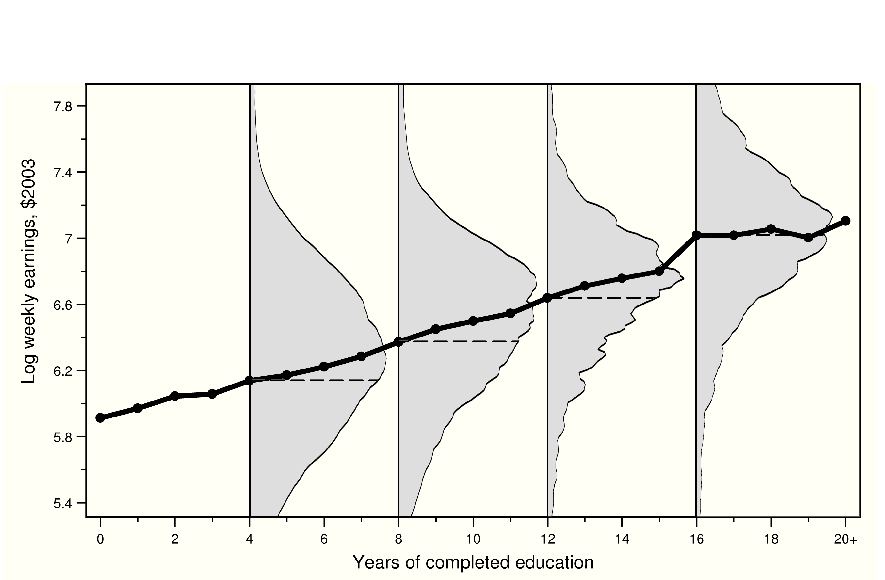
\includegraphics[width=0.65\textwidth]{figures/AP_figure_educacion_salarios.pdf}
            \caption{Esperanza condicional del log salarios semanales dado el nivel educativo. La muestra incluye hombres blancos entre 40 y 49 a\~nos de la muestra del 5\% del Censo 1980 (IPUMS).}
        \end{figure}
    \end{frame}
    % --------------------------------------------------- Slide --
    \subsection{Ley de esperanzas iteradas}
    \begin{frame}
        \frametitle{Ley de esperanzas iteradas (LEI)}
        \begin{itemize}
            \item <1-> Propiedad:
            \begin{align*}
            \E(y)=\E[\E(y|x)]
            \end{align*}
        \end{itemize}
    \end{frame}
    
    \begin{frame}
        \frametitle{Ley de esperanzas iteradas (LEI)}
        \begin{itemize}
            \item Propiedad:
            \begin{align*}
            \E(y)=\E[\E(y|x)]
            \end{align*}
            \bigskip
            \item []  Importante: $\E(y)=\E_x[\E_y(y|x)]$, tomamos primero la esperanza en $y$ manteniendo constante $x$ y luego tomamos la esperanza en $x$.
            \bigskip
            \item [] Demostraci\'on: Utilizar $f_y=\int_x f_{xy}dx$ y $f_{y|x}=f_{xy}/f_{x}$.
        \end{itemize}
    \end{frame}    
          % --------------------------------------------------- Slide --       
        
    \begin{frame} [fragile]
        \frametitle{Ejemplo: LEI $\E(y)=\E[\E(y|x)]$}
     		\begin{table}
     			\small
     			\caption{Funci\'on de esperanza condicional}
     			\begin{tabular}{r c c }
     				\toprule
     				& $\E(ahe|bachelor)$& $\Pr(bachelor)$ \\
     				\midrule
     				$bachelor = 0$    & 15.33  & 0.52 \\
     				$bachelor = 1$    & 22.91  & 0.48 \\
     				\bottomrule	
     			\end{tabular}
     		\end{table}
	\end{frame}

    \begin{frame} [fragile]
        \frametitle{Ejemplo: LEI $\E(y)=\E[\E(y|x)]$}
     		\begin{table}
     			\small
     			\caption{Funci\'on de esperanza condicional}
     			\begin{tabular}{r c c }
     				\toprule
     				& $\E(ahe|bachelor)$& $\Pr(bachelor)$ \\
     				\midrule
     				$bachelor = 0$    & 15.33  & 0.52 \\
     				$bachelor = 1$    & 22.91  & 0.48 \\
     				\bottomrule	
     			\end{tabular}
     		\end{table}
    \begin{align*}
    \E(ahe)=&\E[\E(ahe|bachelor)]\\
    =&\E(ahe|bachelor=0) \Pr(bachelor=0)\\
    &+\E(ahe|bachelor=1) \Pr(bachelor=1)\\
    =& 15.33 \times (1-0.48)  +  22.91 \times 0.48 
    =18.97
    \end{align*}
	\end{frame}

     % --------------------------------------------------- Slide --
    \begin{frame}
        \frametitle{Independencia, independencia en media y correlaci\'on.}
        \begin{itemize}
              		\item \alert{Independencia} 
              		\item [] ${x}\independent{y}$ (independientes) si $\Pr(y|x)=\Pr(y)$.
              		\item [] Una definici\'on equivalente: ${x}\independent{y}$ (independientes) si $\Pr(x,y)=\Pr(y)\Pr(x)$. 
        \end{itemize}    
    \end{frame}
    
         % --------------------------------------------------- Slide --   
    
    \begin{frame}
        \frametitle{Independencia, independencia en media y correlaci\'on.}
        \begin{itemize}
              		\item \alert{Independencia en media} 
              		\item [] $\E(y|x)=\E(y)$.
        \end{itemize}    
    \end{frame}

        % --------------------------------------------------- Slide --

    \begin{frame}
        \frametitle{Independencia, independencia en media y correlaci\'on.}
        \begin{itemize}
    			\item \alert{Covarianza} entre $x,y$: $\Cov(x,y)=\E[(x-\E (x))(y-\E (y))]$
    			\begin{itemize}
    				\item Mide la relaci\'on lineal entre $x$ e $y$.
    				\item Propiedades:
    				\item [] $\Cov(x,y)=\E(xy)-\E (x) \E (y)$
%    			\item [] $\Cov(x,y)=\E[(x-\E(x))y]=\E[(y-\E (y))x]$
%    			\item [] $\Cov(y,y)=\Var(y)$
    				\item [] $\Cov(y,a+bx)=b \Cov(x,y)$
    			\end{itemize}          
        \end{itemize}    
    \end{frame}

        % --------------------------------------------------- Slide --
    \begin{frame}
        \frametitle{Independencia, independencia en media y correlaci\'on.}
        \begin{itemize}
            \item \alert{Independencia en media implica ausencia de correlaci\'on}
            \begin{align*}
            \E(y|x) = \E(y) \implies \Cov(x,y) = 0.
            \end{align*}
        \end{itemize}
    \end{frame}
        
    \begin{frame}
        \frametitle{Independencia, independencia en media y correlaci\'on.}
        \begin{itemize}
            \item \alert{Independencia en media implica ausencia de correlaci\'on}
            \begin{align*}
            \E(y|x) = \E(y) \implies \Cov(x,y) = 0.
            \end{align*}
            \item <1-> Demostraci\'on: Utilice la LEI en
            \begin{align*}
            \E(x y) =\E[x\E(y|x)] = \E(x) \E(y),
            \end{align*}
            y reemplace en la definici\'on de $\Cov(x,y) = \E(x y)-\E(x) \E(y)$.
            \bigskip
            \item <2-> Independencia en media implica ausencia de correlaci\'on con cualquier funci\'on de $x$: \\
            $\E(y|x) = \E(y) \implies \Cov(g(x),y) = 0$ para cualquier funci\'on $g(x)$.
        \end{itemize}
    \end{frame}    

    % --------------------------------------------------- Slide --
    \begin{frame}
        \frametitle{Independencia, independencia en media y correlaci\'on.}
        \begin{itemize}
            \item <1-> \alert{Independencia implica independencia en media}.
            \begin{align*}
            y \independent x \iff f_{y|x}=f_{y} \implies \E(y|x) = \E(y).
            \end{align*}
            Demostraci\'on: Utilice la definici\'on de esperanza condicional.
        \end{itemize}
    \end{frame}
    
    \begin{frame}
        \frametitle{Independencia, independencia en media y correlaci\'on.}
        \begin{itemize}
            \item <1-> \alert{Independencia implica independencia en media}.
            \begin{align*}
            y \independent x \iff f_{y|x}=f_{y} \implies \E(y|x) = \E(y).
            \end{align*}
            Demostraci\'on: Utilice la definici\'on de esperanza condicional.
            \bigskip
            \item <1-> Independencia implica independencia en todos los momentos de $y$.
            En particular, $y \independent x  \implies \Var(y|x) = \Var(y)$.
            
            \bigskip
            
            Demostraci\'on: Utilice la definici\'on de la varianza condicional $\Var(y|x)=\E[(y-\E(y|x))^2|x]$.
        \end{itemize}
    \end{frame}
        
    % --------------------------------------------------- Slide --
    \begin{frame}
        \frametitle{Independencia, independencia en media y correlaci\'on.}
        \begin{itemize}
            \item <1-> Resumen:\\
            $y \independent x \implies \E(y|x) = \E(y) \implies \Cov(x, y) = 0$
            \uncover <2->{$\Cov(y, x) = 0   \centernot \implies  \E(y|x) = \E(y) \centernot \implies  y \independent x $}
            \item <3-> En la ayudant\'ia se ven casos en donde: 
            \begin{enumerate}
              \item $\E(y|x) = \E(y) \centernot \implies  y \independent x $, 
              \item $\Cov(y, x) = 0   \centernot \implies  \E(y|x) = \E(y) $
            \end{enumerate} 
        
        \end{itemize}
    \end{frame}
    % --------------------------------------------------- Slide --
    \subsection{Descomposici\'on}
    \begin{frame}
        \frametitle{Descomposici\'on utilizando la esperanza condicional}
        \begin{itemize}
            \item <1-> Siempre podemos descomponer a la variable aleatoria $y$ en
            \begin{align*}
            y = \E(y|x) + u,
            \end{align*}
            donde $u$ es independiente en media de $x$, es decir $\E(u|x)=0$.
        \end{itemize}            
    \end{frame}
    
    \begin{frame}
        \frametitle{Descomposici\'on utilizando la esperanza condicional}
        \begin{itemize}
            \item <1-> Siempre podemos descomponer a la variable aleatoria $y$ en
            \begin{align*}
            y = \E(y|x) + u,
            \end{align*}
            donde $u$ es independiente en media de $x$, es decir $\E(u|x)=0$.
            
            \bigskip
            
            Demostraci\'on: Reemplace $u=y-\E(y|x)$ en $\E(u|x)$.
            
            \bigskip
            
            \item <1-> Interpretaci\'on: Una variable aleatoria $y$ se puede descomponer en una parte ``explicada por $x$'' y otra parte que no depende de $x$.
        \end{itemize}
        % Este resultado es \'util como justificaci\'on de la esperanza condicional como momento de inter\'es. y_i depende de muchos elementos aleatorios, pero nosotros estamos interesados en medir el efecto sistem\'atico de x_i en y_i(en la media de y_i)
    \end{frame}
    
    % --------------------------------------------------- Slide --
    \subsection{Mejor predicci\'on}
    \begin{frame}
        \frametitle{La esperanza condicional es el mejor predictor de $y$}
        \begin{itemize}
            \item <1-> La esperanza condicional es la funci\'on de $x$ que \alert{minimiza el error cuadr\'atico medio de predicci\'on}, es decir
            \begin{align*}
            \E(y|x) = \arg \min_{m(x)} \E[(y-m(x))^2].
            \end{align*}
        \end{itemize}
        % Si solamente estamos interesados en predicci\'on, la esperanza condicional es un excelente predictor.
        % Si utiliamos otro criterio para evaluar la mejor predicci\'on, podemos obtener otro predictor \'optimo. Por ejemplo, si nos interesa minimizar el error absoluto medio de predicci\'on, el predictor \'optimo es la mediana condicional.
    \end{frame}
    
    \begin{frame}
        \frametitle{La esperanza condicional es el mejor predictor de $y$}
        \small
        \begin{itemize}
            \item <1-> La esperanza condicional es la funci\'on de $x$ que \alert{minimiza el error cuadr\'atico medio de predicci\'on}, es decir
            \begin{align*}
            \E(y|x) = \arg \min_{m(x)} \E[(y-m(x))^2].
            \end{align*}
            
            \bigskip
            
            \item <1-> Demostraci\'on:
            \begin{align*}
            \E[(y-m(x))^2] & =    \E\{[(y-\E(y|x))-(m(x)-\E(y|x))]^2\} \\
            & =    \E\{(y-\E(y|x))^2+(m(x)-\E(y|x))^2 \\
            &      -2(y-\E(y|x)) (m(x)-\E(y|x))\} \\
            & =    \E[(y-\E(y|x))^2]+\E[(m(x)-\E(y|x))^2]\\
            & \geq \E[(y-\E(y|x))^2],
            \end{align*}
            donde en la tercer l\'inea utilizamos la LEI para demostrar que $\E[(y-\E(y|x)) (m(x)-\E(y|x))]=0$.
        \end{itemize}
        % Si solamente estamos interesados en predicci\'on, la esperanza condicional es un excelente predictor.
        % Si utiliamos otro criterio para evaluar la mejor predicci\'on, podemos obtener otro predictor \'optimo. Por ejemplo, si nos interesa minimizar el error absoluto medio de predicci\'on, el predictor \'optimo es la mediana condicional.
    \end{frame}
        
    % --------------------------------------------------- Slide --
    \subsection{Descomposici\'on de varianza}
    \begin{frame}
        \frametitle{Descomposici\'on de varianza}
        \begin{itemize}
            \item <1-> La varianza de la variable aleatoria $y$ se puede descomponer como
                \begin{align*}
                    \Var(y) = & \Var(\E(y|x)) + \E(\Var(y|x)) ,&(1)\\
                              = & \Var(\E(y|x)) + \E(u^2), &(2)
                \end{align*}
            donde $\Var(y|x)=\E[(y-\E(y|x))^2|x]$ es la varianza de  $y$ condicional en $x$.
                 \end{itemize}
        % Utilizaremos este resultado (o similar) para hablar de bondad de ajuste, que parte de la variabilidad de y es explicada por la media condicionada.
    \end{frame}
    % --------------------------------------------------- Slide --
    \begin{frame}
        \frametitle{Descomposici\'on de varianza}
        \begin{itemize}
            \item Demostraci\'on: Para (1) 
            \begin{align*}
                \Var(y) & = \E[(y-\E(y))^2],\\
                          & = \E\{[(y-\E(y|x))+(\E(y|x)-\E(y))]^2\}, \\
                          & = \E[(y-\E(y|x))^2]         + \E[(\E(y|x)-\E(y))^2], \\
                          & = \E[\E((y-\E(y|x))^2|x)] + \Var(\E(y|x)),\\
                          & = \E(\Var(y|x))               + \Var(\E(y|x)),
            \end{align*}
            donde utilizamos la LEI en la tercer y cuarta l\'inea.
        \end{itemize}
        % Utilizaremos este resultado (o similar) para hablar de bondad de ajuste, que parte de la variabilidad de y es explicada por la media condicionada.
    \end{frame}
       % --------------------------------------------------- Slide --
    \begin{frame}
        \frametitle{Descomposici\'on de varianza}
        \begin{itemize}
            \item  Demostraci\'on: Para (2), utilizamos $y=\E(y|x)+u$ para escribir 
            \begin{align*}
                \Var(y|x) & = \Var(u|x),\\
                              & = \E(u^2|x).
            \end{align*}
            Por lo tanto,
            \begin{align*}
                \E(\Var(y|x)) & = \E(\E(u^2|x)),\\
                                  & = \E(u^2),
            \end{align*}
            utilizando la LEI.
        \end{itemize}
    \end{frame}
    % --------------------------------------------------- Slide --
    
    \section{Modelo de regresi\'on lineal}
    \subsection*{Definici\'on}
    \begin{frame}
        \frametitle{Modelo de Regresi\'on Lineal : $\LP(y|x)=x'\beta$}
        \begin{itemize}
            \item <1-> \alert{Mejor predictor lineal}: Es la funci\'on lineal $\LP(y|x)=x'\beta$ que minimiza el error cuadr\'atico medio de predicci\'on \alert{entre las funciones lineales en $x$}, es decir
            \begin{align*}
            \beta = \arg \min_b \E[(y-x'b)^2],
            \end{align*}
            donde $y$ es un escalar, $x=(x_{1},...,x_{K})'$ es un vector de $K \times 1$ (casi siempre incluye una constante), y $\beta=(\beta_{1},...,\beta_{K})'$ es un vector de $K \times 1$.
          \end{itemize}
    \end{frame}

    \begin{frame}
        \frametitle{Ejemplo: Tamaño de clase y notas}
        \begin{figure}
            
\includegraphics[width=0.75\textwidth]{figures/test_score_class_size.png}
        \end{figure}
    \end{frame}
    
    \begin{frame}
        \frametitle{¿Cómo se obtiene $\beta$ de $\LP(y|x)=x'\beta$?}
        \begin{itemize}
        		\item <2->
                Utilizando las condiciones de primer orden
                \begin{align*}
                \frac{\partial\E[(y-x'b)^2]}{\partial b}&=2\E[x(y-x'\beta)]=0 \\
                \implies \beta&= \E(xx')^{-1}\E(x y).
                \end{align*}
        		\item <2->
                Si $\E(x x')$ es no singular, entonces $\beta$ existe y es \'unica.
            \item <2->  \alert{M\'etodo de momentos}: $\beta$ tal que  
            $\E[x(y-x'\beta)]=0$.
            \end{itemize}
    \end{frame}
    
    % Todo lo que estamos hablando es en la poblaci\'on.
    % Identificaci\'on: Escribir los par\'ametros de inter\'es como funci\'on de momentos poblacionales.
    % Condiciones de segundo orden para un m\'inimo \E(xx') semidefinida positiva. Si incluye la constante,\Var(x)=\E(xx') por lo tanto \Var(a'x)=a'\E(xx')a>=0
    % --------------------------------------------------- Slide --
    
    \begin{frame}
        \frametitle{Ejemplo: Modelo de regresi\'on simple}
        \begin{itemize}
            \item Si $x=(1, x_{1})$, entonces $\LP(y|x)=\beta_0+\beta_1x$ con
            \begin{align*}
            \beta_1 &= \frac{\Cov(x_{1}, y)}{\Var(x_{1})}, \text{ y}\\
            \beta_0 &= \E(y)-\beta_1\E(x_{1}).
            \end{align*}
            \bigskip
        \end{itemize}
    \end{frame}

    % --------------------------------------------------- Slide --
    \subsection{Descomposici\'on}
    \begin{frame}
        \frametitle{Descomposici\'on utilizando el modelo de regresi\'on}
        \begin{itemize}
            \item <1-> Siempre podemos descomponer a la variable aleatoria $y$ en
            \begin{align*}
            y = x'\beta + u,
            \end{align*}
            donde $u$ cumple que $\E(xu)=0$.
        \end{itemize}
    \end{frame}
 
        % --------------------------------------------------- Slide --
    \begin{frame}
        \frametitle{Descomposici\'on utilizando el modelo de regresi\'on}
        \begin{itemize}
            \item <1-> Siempre podemos descomponer a la variable aleatoria $y$ en
            \begin{align*}
            y = x'\beta + u,
            \end{align*}
            donde $u$ cumple que $\E(xu)=0$.
            
            \item <1-> Demostraci\'on: $\E(xu)=\E(x(y-x'\beta))=0$ que se cumple por la definici\'on de modelo de regresi\'on por el m\'etodo de momentos.
            \bigskip
            
           \item <1-> {$x$ casi siempre incluye una constante, entonces $\E(u)=0$. Por lo tanto si $\E(xu)=0$ entonces $\Cov(x,u)=0$.}
        \end{itemize}
    \end{frame}
    
    \begin{frame}
        \frametitle{Descomposici\'on utilizando el modelo de regresi\'on}
        \begin{itemize}
            \item <1-> Siempre podemos descomponer a la variable aleatoria $y$ en
            \begin{align*}
            y = x'\beta + u,
            \end{align*}
            donde $u$ cumple que $\E(xu)=0$.           
            \item <1-> Interpretaci\'on: Una variable aleatoria $y$ se puede descomponer en una parte ``explicada por $x$'' y otra parte no correlada con $x$.
            \item <2-> Propiedad: Si denotamos el valor predicho de $y$ dado $x$ como $\hat y=\LP(y|x)=x'\beta$ entonces $\E(\hat y u)=0$ y si $x$ incluye la constante $\Cov(\hat y, u)=0$.
        \end{itemize}
    \end{frame}
    
    % --------------------------------------------------- Slide --
    \subsection{Regresi\'on particionada}
    \begin{frame}
        \frametitle{Regresi\'on particionada}
        \begin{itemize}
            \item <1-> Dado el modelo de regresi\'on m\'ultiple
            \begin{align*}
            y = \beta_0+\beta_1x_{1}+...+\beta_k x_{k} +...+\beta_K x_{K}+ u.
            \end{align*}
            Podemos recuperar $\beta_k$ a partir de la regresi\'on simple entre $y$ y $\tilde x_{k}$, el residuo de la regresi\'on de $x_{k}$ en el resto de las variables explicativas $x_1,...,x_{k-1},x_{k+1},...,x_K$:
            \begin{align*}
            \beta_{k} = \frac{\Cov(\tilde x_{k},y)}{\Var(\tilde x_{k})},
            \end{align*}
            donde
            \begin{align*}
            x_{k} = \sum_{j\neq k} \gamma_j \, x_{j}+\tilde x_{k} =\hat x_{k}+\tilde x_{k}.
            \end{align*}
            Ejemplo: Dado $y=\beta_0+\beta_1 x_1+\beta_2 x_2+u$, tenemos $x_1=\gamma_0+\gamma_1x_2+\tilde x_1$ y $y+\delta_0+\delta_1 \tilde x_1+e$. Entonces $\delta_1=\beta_1$.
        \end{itemize}
    \end{frame}
    % --------------------------------------------------- Slide --
    \begin{frame}
        \frametitle{Regresi\'on particionada}
        \begin{align*}
        \beta_{k} = \frac{\Cov(\tilde x_{k},y)}{\Var(\tilde x_{k})}
        \end{align*}
        \begin{itemize}
            \item <1-> Interpretaci\'on: $\beta_k$ mide el efecto de $x_k$ sobre $y$, una vez que filtramos (controlamos por) el efecto de las dem\'as variables explicativas.
        \end{itemize}
    \end{frame}
    % Esta interpretaci\'on esta relacionada a la posibilidad de que el modelo de regresi\'on mida un efecto causal. En el caso del tama\~no de clase, dado que no tenemos datos experimentales, queremos ver el efecto del tama\~no de clase en rendimiento acad\'emico controlando por diferencias socio-econom\'omicas de los estudiantes.
    % --------------------------------------------------- Slide --
    \begin{frame}
        \frametitle{Regresi\'on particionada}
        \begin{itemize}
            \item <1-> Demostraci\'on: 
            \begin{align*}
            \frac{\Cov(\tilde x_{k},y)}{\Var(\tilde x_{k})} = \frac{\Cov(\tilde x_{k},\beta_0+\beta_1x_{1}+...+\beta_k x_{k} +...+\beta_K x_{K}+ u)}{\Var(\tilde x_{k})}.
            \end{align*}
            \begin{enumerate}
                \item[(1)] $\Cov(\tilde x_{k},x_{j})=0$ para todo $j\neq k$, por construcci\'on,
                \item[(2)] $\Cov(\tilde x_{k},u)=0$ porque $u$ no est\'a correlado con $x$'s y $\tilde x_{k}$ es una funci\'on lineal de $x$'s.
            \end{enumerate}
            Entonces,
            \begin{align*}
            \frac{\Cov(\tilde x_{k},y)}{\Var(\tilde x_{k})} & = \beta_k\frac{\Cov(\tilde x_{k},x_{k})}{\Var(\tilde x_{k})},\\
            & = \beta_k\frac{\Cov(\tilde x_{k},\hat x_{k}+\tilde x_{k})}{\Var(\tilde x_{k})},\\
            & = \beta_k\frac{\Cov(\tilde x_{k},\tilde x_{k})}{\Var(\tilde x_{k})},\\
            & = \beta_k.
            \end{align*}
        \end{itemize}
    \end{frame}
    % --------------------------------------------------- Slide --
    \subsection{Justificaci\'on de utilizar el modelo de regresi\'on}
    \begin{frame}
    	\frametitle{Justificaci\'on de utilizar el modelo de regresi\'on como aproximaci\'on a la esperanza condicional.}
    	\begin{itemize}
       		\bigskip
    		\item Si \alert{esperanza condicional es lineal} entonces el modelo de regresi\'on coincide con la esperanza condicional.
    		\item  El modelo de regresi\'on es el \alert{mejor predictor lineal de $y$}.
    		\item El modelo de regresi\'on es la \alert{mejor aproximaci\'on lineal a la esperanza condicional}.
    	\end{itemize}
    \end{frame}
    % --------------------------------------------------- Slide --
    \begin{frame}
        \frametitle{Esperanza condicional es lineal}
        \begin{itemize}
            \item <1-> Si la esperanza condicional es lineal entonces coincide con el modelo de regresi\'on.
            \bigskip
            \item <2->[] Demostraci\'on: $\E(y|x) = x'\beta^*$. \\
            Por la propiedad de descomposici\'on podemos escribir $y=\E(y|x)+u$ donde $\E(u|x)=0$. Esto implica $\E[x(y-\E(y|x))]=0$, entonces
            \begin{align*}
            \E[x(y-\E(y|x))] & = \E[x(y-x'\beta^*)] =0.
            \end{align*}
            De donde,
            \begin{align*}
            \beta^*= \E(xx')^{-1}\E(xy)=\beta.
            \end{align*}
            \item <3-> \alert{Ejemplos}: 
            \begin{enumerate}
                \item [(1)] $(y, x)$ se distribuyen conjuntamente normal,
                \item [(2)] Modelos saturados. Ejemplo: Cuando $x$ es binaria, $\E(y|x)=\E(y|x=0)+[\E(y|x=1)-\E(y|x=0)]x$ es lineal.
            \end{enumerate}
        \end{itemize}
    \end{frame}
    % --------------------------------------------------- Slide --
    \begin{frame}
        \frametitle{Mejor predicci\'on lineal}
        \begin{itemize}
            \item <1-> El modelo de regresi\'on lineal es el mejor predictor lineal de $y$ dado $x$.
        \end{itemize}
    \end{frame} 
    % --------------------------------------------------- Slide --
   \begin{frame}
        \frametitle{Mejor aproximaci\'on lineal a la esperanza condicional}
        \begin{itemize}
            \item  El modelo de regresi\'on lineal es la mejor aproximaci\'on lineal a la esperanza condicional. Es decir,
            \begin{align*}
            \beta = \arg \min_b \E[(\E(y|x)-x'b)^2]
            \end{align*}
        \end{itemize}
    \end{frame} 
    % Mejor justificaci\'on del modelo de regresi\'on
    % Puede ser un buen predictor de la esperanza condicional pero no tan buen predictor de efcectos parciales para algunos valores de x. Por esto es importante, tener en cuenta efectos no lineales con interacciones, cuadrados, dummies, logaritmos.
                
    % --------------------------------------------------- Slide --
    
    \begin{frame}
        \frametitle{Mejor aproximaci\'on lineal a la esperanza condicional}
        \begin{itemize}
            \item <1-> El modelo de regresi\'on lineal es la mejor aproximaci\'on lineal a la esperanza condicional. Es decir,
            \begin{align*}
            \beta = \arg \min_b \E[(\E(y|x)-x'b)^2]
            \end{align*}
            \item <1-> [] Demostraci\'on: 
            \begin{align*}
            \E[(y-x'b)^2]=&\E\{[(y-\E(y|x))+(\E(y|x)-x'b)]^2\}\\
            =&\E\{(y-\E(y|x))^2+(\E(y|x)-x'b)^2\\
            &+2(y-\E(y|x))(\E(y|x)-x'b)\}\\
            =&\E[(y-\E(y|x))^2]+\E[(\E(y|x)-x'b)^2].
            \end{align*}
            El primer t\'ermino no depende de $b$, entonces $\beta=\arg \min_b\E[(y-x'b)^2] \iff \beta=\arg \min_b\E[(\E(y|x)-x'b)^2]$.
        \end{itemize}
    \end{frame} 
    % Mejor justificaci\'on del modelo de regresi\'on
    % Puede ser un buen predictor de la esperanza condicional pero no tan buen predictor de efcectos parciales para algunos valores de x. Por esto es importante, tener en cuenta efectos no lineales con interacciones, cuadrados, dummies, logaritmos.
    % --------------------------------------------------- Slide --
    \begin{frame}
        \frametitle{Ejemplo: Educaci\'on y salarios}
        \begin{figure}
            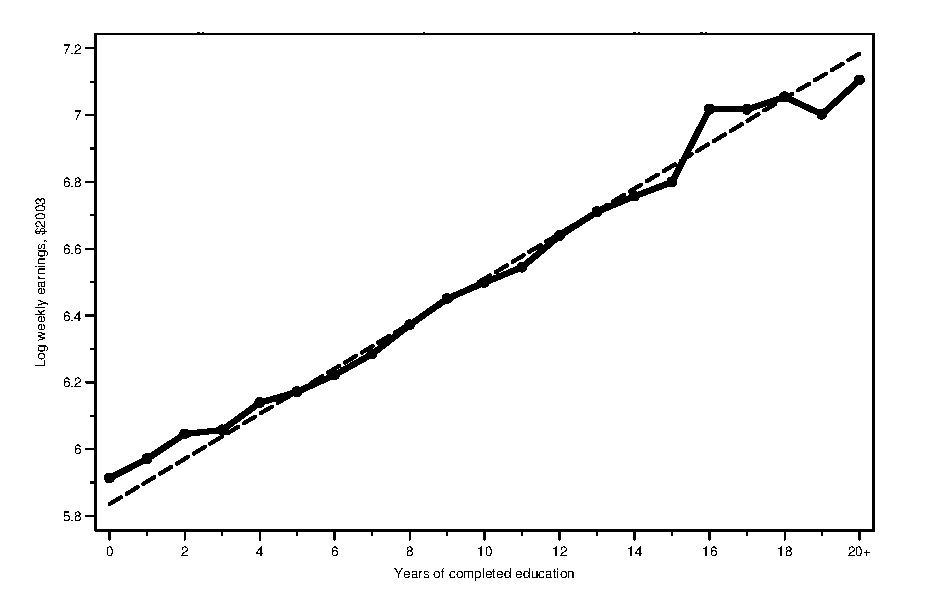
\includegraphics[width=0.65\textwidth]{figures/AP_figure_educacion_salarios_regresion.pdf}
            \caption{Regresi\'on y esperanza condicional del log salarios semanales en el nivel educativo. La muestra incluye hombres blancos entre 40 y 49 a\~nos de la muestra del 5\% del Censo 1980 (IPUMS).}
        \end{figure}
    \end{frame}
    % --------------------------------------------------- Slide --
    \subsection{Descomposici\'on de varianza}
    \begin{frame}
        \frametitle{Descomposici\'on de varianza en regresi\'on}
        \begin{itemize}
            \item <1-> Si $x$ incluye una constante, la varianza de la variable aleatoria $y$ se puede descomponer como
            \begin{align*}
            \Var(y) = & \Var(x'\beta) + \E(u^2).
            \end{align*}
            Demostraci\'on: Utilice la descomposici\'on de $y=x'\beta+u$ y  $\E(u x)=\Cov(u,x)=0$.
            \item <2-> \alert{Coeficiente de determinaci\'on}: $R^2$,
            \begin{align*}
            R^2 & = 1-\frac{\E(u^2)}{\Var(y)}.
            \end{align*}
            \item <2-> [] Indicador de la bondad de ajuste del modelo de regresi\'on.
        \end{itemize}
    \end{frame}

    % --------------------------------------------------- Slide --
    \begin{frame}[label=figure2]
        \frametitle{Ejemplo: Educaci\'on y salarios en US}
        \begin{figure}
            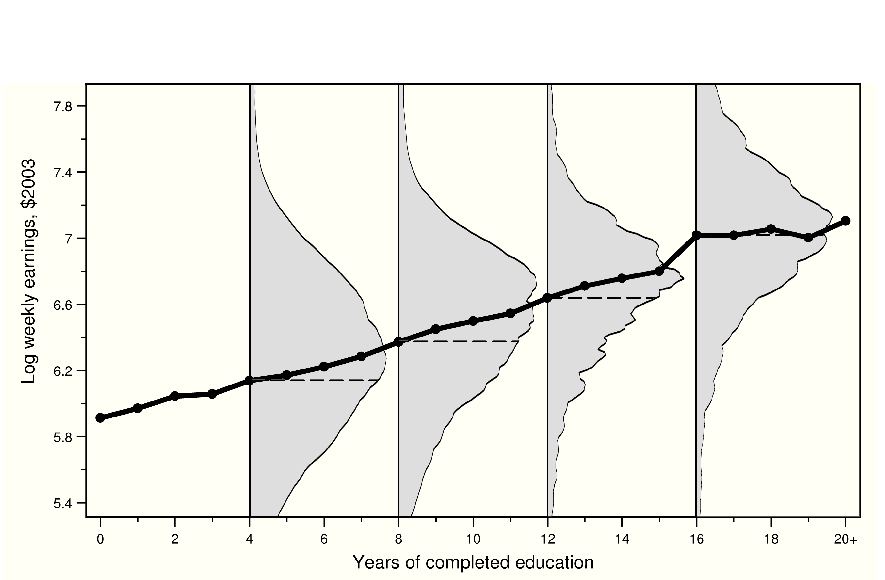
\includegraphics[width=0.65\textwidth]{figures/AP_figure_educacion_salarios.pdf}
            \caption{Esperanza condicional del log salarios semanales dado el nivel educativo. La muestra incluye hombres blancos entre 40 y 49 a\~nos de la muestra del 5\% del Censo 1980 (IPUMS).}
        \end{figure}
    \end{frame}
    % --------------------------------------------------- Slide --
    \begin{frame}
        \frametitle{Ejemplo: Educaci\'on y salarios en Chile}
        \begin{figure}
            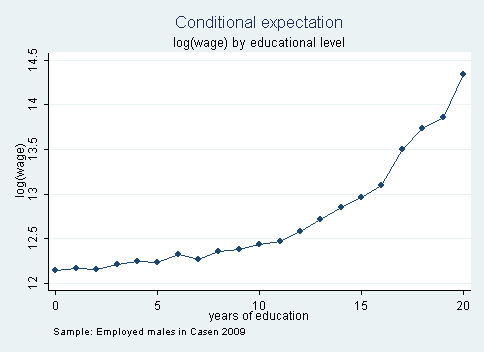
\includegraphics[width=0.6\textwidth]{figures/cond_expec_wage_educ1.png}
            \caption{Esperanza condicional del log de salarios dado el nivel educativo. La muestra incluye hombres trabajadores en Casen 2009. \hyperlink{back2}{\beamergotobutton{back}}}
        \end{figure}
    \end{frame}
    % --------------------------------------------------- Slide --
    \begin{frame}[label=figure3]
        \frametitle{Ejemplo: Educaci\'on y salarios en US}
        \begin{figure}
            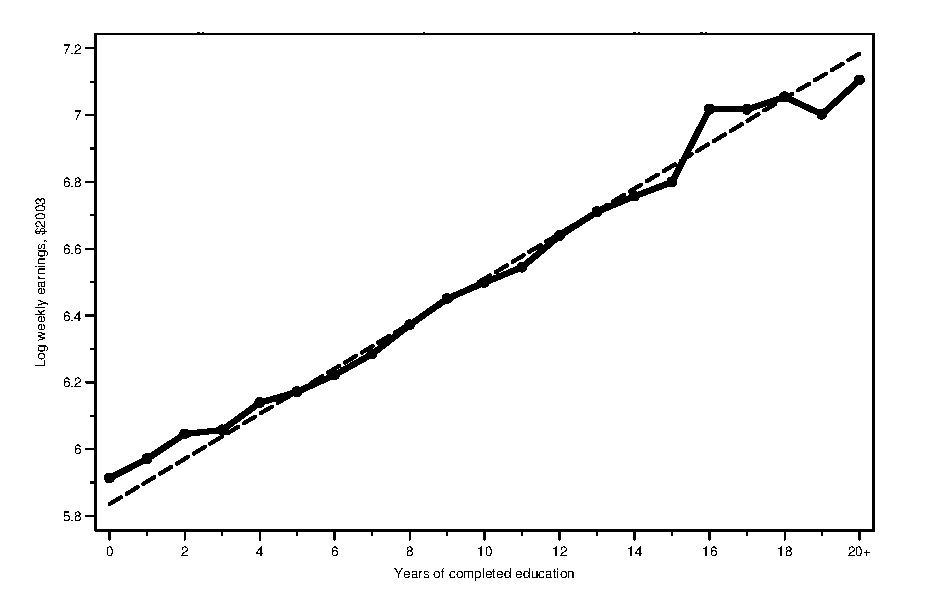
\includegraphics[width=0.65\textwidth]{figures/AP_figure_educacion_salarios_regresion.pdf}
            \caption{Regresi\'on y esperanza condicional del log salarios semanales en el nivel educativo. La muestra incluye hombres blancos entre 40 y 49 a\~nos de la muestra del 5\% del Censo 1980 (IPUMS).}
        \end{figure}
    \end{frame}
    % --------------------------------------------------- Slide --
    \begin{frame}
        \frametitle{Ejemplo: Educaci\'on y salarios en Chile}
        \begin{figure}
            
\includegraphics[width=0.70\textwidth]{figures/cond_expec_wage_educ2.png}
            \caption{Regresi\'on y esperanza condicional del log salarios semanales en el nivel educativo. La muestra incluye hombres trabajadores en Casen 2009.}
        \end{figure}
    \end{frame}
    % --------------------------------------------------- Slide --
    \begin{frame}
        \frametitle{Ejemplo: Educaci\'on y salarios en Chile}
        \begin{figure}
            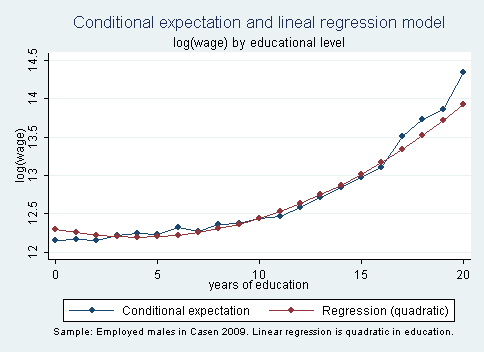
\includegraphics[width=0.6\textwidth]{figures/cond_expec_wage_educ3.png}
            \caption{Regresi\'on y esperanza condicional del log salarios semanales en el nivel educativo. La muestra incluye hombres trabajadores en Casen 2009. \hyperlink{back3}{\beamergotobutton{back}}}
        \end{figure}
    \end{frame}
\end{document}
